\documentclass{article}
\usepackage[utf8]{inputenc}
\usepackage{float}
\usepackage{xcolor}
\usepackage{graphicx}
\usepackage{amsmath}
\usepackage{amssymb}
\usepackage{placeins}
\usepackage{booktabs}
\usepackage{caption}
\usepackage{makecell}

\usepackage{hyperref}
\usepackage{textcomp}
\hypersetup{
    colorlinks=true,
    linkcolor=blue,
    filecolor=magenta,      
    urlcolor=blue,
}

\title{Scientific Computing - Molecular dynamics \\ Group F}
\newcommand{\subtitle}{Problem sheet 4}
\author{
    Jimin Kim \\
    Christian Nix \\
    Noah Schlenker
}
\date{\today}

\begin{document}

\maketitle

\begin{center}
    \LARGE \subtitle{}
\end{center}

\section{Pull request}
\label{sec:pr}
The pull request can be found \href{https://github.com/noahpy/MolSim-SS24/pull/42}{here}.

\section{Bug Fixes and Implementation of missing features}
\label{sec:fix}

    \begin{itemize}
        \item We addressed several issues and incorporated the requested functionalities into the previous assignment.
        \item A check for the cutoff radius in particle calculations has been added.
        \item We implemented the removal of particles from calculations and ParaView visualization if they move beyond the outflow boundaries (see previous report for our prior handling of outflow boundaries):
        \begin{itemize}
            \item Particles now possess a boolean attribute, \texttt{active}, indicating whether the particle is out of bounds.
            \item Instead of performing costly operations and reallocations to delete particles, we manage them using simple flags.
            \item The refactored project structure allows us to modify particle container iterators without disrupting the functionalities of previous assignments or necessitating extensive code adjustments.
        \end{itemize}
        \item We corrected errors affecting certain particles at the corners of reflective boundaries.
        \item The simulation refactoring to allow selection between different simulation options without creating a new simulation class will be implemented in the next assignment. This decision was made to prioritize the new tasks and due to time constraints.
    \end{itemize}

All new features have been tested with their according Unit tests (see \texttt{tests}).

\section{Thermostat}
\label{sec:thermo}

    \begin{itemize}
        \item We introduced a new class, \texttt{Thermostat}, in \texttt{src/physics} for temperature calculations to adjust the velocities of all particles in the container.
        \item The temperature update process follows the calculation steps outlined in the assignment sheet.
        \item To optimize temperature calculations, we excluded the divisions by 2 in the calculation of $E_{kin}$, as the energy is multiplied by 2 in the current temperature calculation:
        \begin{align}
            T_{current} &= \frac{2 \cdot \left(\sum_{i=1}^{\#particles} \frac{m_i \langle v_i, v_i \rangle}{2}\right)}{\#dimensions\ \cdot\ \#particles} \\
            &= \frac{2 \cdot \frac{1}{2}\ \left(\sum_{i=1}^{\#particles} m_i \langle v_i, v_i \rangle\right)}{\#dimensions\ \cdot\ \#particles} \\
            &= \frac{\sum_{i=1}^{\#particles} m_i \langle v_i, v_i \rangle}{\#dimensions\ \cdot\ \#particles}
        \end{align}
        \item This class also provides a function for temperature initialization utilizing the \texttt{maxwellBoltzmannDistributedVelocity} function.
        \item The step counter for the frequency of temperature updates is managed within the simulation layer, as it controls the frequency of update operations in our project structure.
    \end{itemize}
    
    
\section{Rayleigh-Taylor instability Simulation}
\label{sec:rayleigh}

\subsection{Periodic Boundary}
\label{sec:rayleigh:periodic}
\begin{itemize}
    \item Our boundary interface specifies two functions for handling boundary conditions: \texttt{preUpdateBoundaryHandling} and \texttt{postUpdateBoundaryHandling}
    \item \texttt{preUpdateBoundaryHandling}
    \begin{itemize}
        \item This is executed before any forces are calculated. Thus, this call is used to add all required halo particles
        \item To do this, a \texttt{map<CellIndex, vector<pair<coordinateShift, coordinateShift>>>} is precomputed
        \item The map resolves a \texttt{CellIndex} of the \texttt{CellGrid} to a list of manipulations to perform on a particles position and CellIndex
        \item E.g. if the particles is located in the top left corner and is leaving the domain to the left, one shift component contains the coordinate shift to be added to the particle's position (moving it to the top right cell), while the other component contains the coordinate shift for the cell (CurrentCellIndex+Shift = NewCellIndex, i.e. NewCellIndex = Top-Right)
        \item To not apply multiple shifts (e.g. when particle is in corner and belongs to two periodic boundaries), we define an order of the sides
        \item E.g. when calculation the shifts for the top-left cell, the left boundary will handle all shifts, while the top boundary will do no moves on that cell
    \end{itemize}
    \item \texttt{postUpdateBoundaryHandling}
    \begin{itemize}
        \item This is called after all updates to the particles (calcf, calcv, clacx)
        \item Here, all inserted halo particles will be removed. This is legal, as we inserted halo particles after the last update cells and thus no particles from inside the domain can have crossed into a halo cell and vice versa (in terms of being assigned to that cell)
        \item Then all particles in the boundary cells of the periodic boundary will be looked at
        \item If their position has changed outside the domain, the shift for that side of the boundary will be applied (i.e. if particle is on the crossed to the left, it will be moved by the size of the domain to the right)
        \item Because the order the periodic boundaries are applied in is not known to the boundary during the \texttt{postUpdateBoundaryHandling} call, a way must be found to know when all periodic boundaries have applied their shift, to assign the particle to the new cell
        \item A nice way we found, was that the particle will only every get back into the domain after all periodic boundaries that influence it are completed
        \item E.g. if the particle is in the top left corner, a shift to the right will still move it to a halo cell and only the shift down will place it back into the domain
    \end{itemize}
\end{itemize}

    \begin{itemize}
        \item XML related parser and reader have been adjusted to accommodate new parameters, such as particle types in clusters.
        \item A new force calculation function, \texttt{force\_mixed\_LJ\_gravity\_lc}, incorporating an additional gravitational force, has been implemented.
        \item We introduced a new simulation class, \texttt{MixedLJSimulation}, for simulating different particle types simultaneously:
        \begin{itemize}
            \item The Lennard-Jones parameters, following to the Lorentz-Berthelot mixing rule, are determined in the constructor of the class.
            \item $\epsilon$ and $\sigma$ values of all type combinations, along with alphas, betas and gammas, are computed and inserted upon simulation initialization for optimization purposes (see last report).
            \item The simulation checks if particles are outside the domain during initialization.
            \item We included the thermostat, so that the temperature initialization is handled during simulation setup.
        \end{itemize}
        \item The added section of the project UML diagram can be seen here Fig.\ \ref{fig:uml}.
        \item Running the simulation revealed a couple observations:
        \begin{itemize}
            \item The falling particles bounce noticeably, when the two particle layers collide.
            \item Initially, the top liquid doesn't mix into the bottom layer evenly, but forms several drops as it sinks.
        \end{itemize}
    \end{itemize}

\begin{figure}[H]
    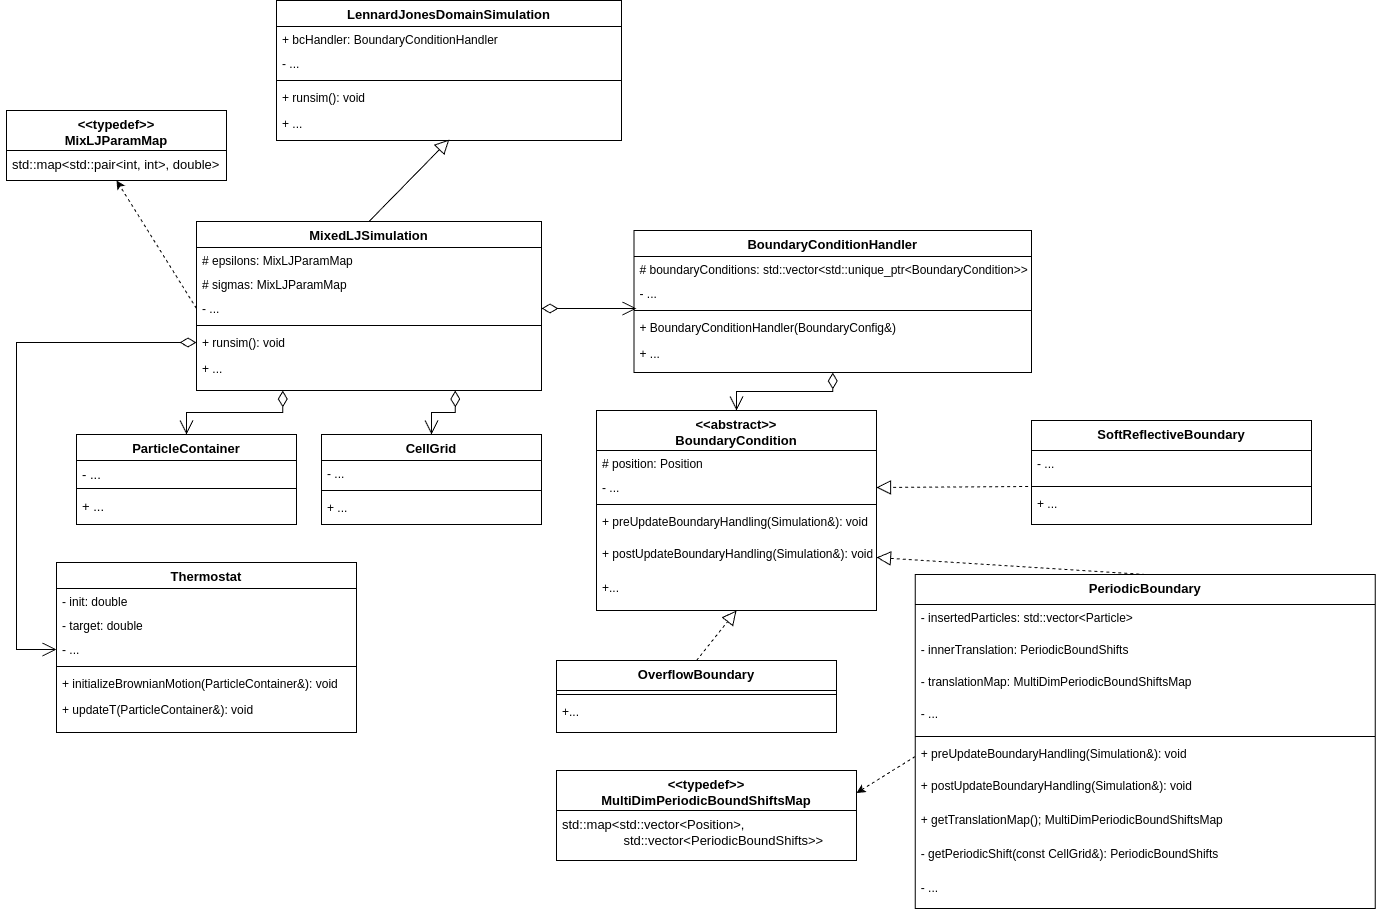
\includegraphics[width=1.25\textwidth]{../../res/UML4v2.drawio}
    \caption{UML diagram extension.}
    \label{fig:uml}
\end{figure}

\section{Falling drop - Liquid}
\label{sec:drop}

    \begin{itemize}
        \item Checkpoints were implemented to acquire the equilibrated fluid:
        \begin{itemize}
            \item Checkpointing is realized through saving a simulation state in the same XML format as the input files. This allows us to easily add clusters / modify parameters after equilibration. To save individual particles, we decided to save their mass, velocity, force and type respectively in a list format. Additionally, we introduced a format which maps types to sigma and epsilon.
            \item We implemented a \texttt{XmlWriter} for writing the formatted files (see \texttt{src/io/fileWriter}), which can be activated via the command line argument \texttt{-w 2}.
        \end{itemize}
    \item We first applied the thermostat to the simulation, which showed a slow descend of the drop and a calm assimilation into the fluid below due to velocity adjustments. Due to the calm impact, one can observe interesting wave patterns reflecting from the boundaries! :)
        \item Without temperature regulation, the drop falls rapidly and splashes violently into the liquid. One can still obsevere a big wave of particles reflecting from the side boundaries, which was a great sight!
        \item Running the simulation with periodic boundaries showed negligible differences. This is likely because particles at the edges collided similarly to reflecting boundaries, given that the drop falls into the liquid center.    \end{itemize}


\section{Performance Measurment}
\label{sec:perf}
    
\begin{itemize}
    \item We modified our project as suggested to measure the runtime of the main loop, the time per iteration, and the MUP/S (Molecule update per second) where we define a molecule update as the molecule receiving its new position at the end of an iteration i.e. after one iteration \textit{\#active particles} molecule updates have been performed.
    \item The measurements were conducted on a large scenario ($\geq 10000\ molecules$) with I/O operations disabled. For this we used the big Rayleigh with $t_{end} = 25$. 
    \item We profiled the code using \texttt{gprof} on the small Rayleigh. The data for profiling is presented in Tab.\ \ref{table:data}.
    \item This data indicates that the force calculation routine is the most time-consuming section, accounting for 77.07\% of the total runtime (\texttt{lj\_calc(...)} is part of force calculation).
    \item The runtime of the small Rayleigh-Taylor simulation on the cluster (cm2\_tiny) can be viewed here Tab.\ \ref{table:small_raileigh}. Unfortunately, cluster scheduling did not leave us the time to run the bigger experiments on the cluster to get measurements from there.
    \item We ran the full Rayleigh-Taylor simulation locally with the following specs\ \ref{table:specs} and the runtime seen here\ \ref{table:rayleigh_base}.
\end{itemize}

\begin{table}[H]
    \centering
    \resizebox{1.2\textwidth}{!}{
        \begin{tabular}{|c|c|c|c|c|c|l|}
            \hline
            \% Time & Cumulative Seconds & Self Seconds & Calls & ms/call Self & ms/call Total & Name \\ \hline
            67.12 & 65.33 & 65.33 & 50,001 & 1.31 & 1.79 & \makecell[l]{force\_mixed\_LJ\_gravity\_lc\\(Simulation const\&)} \\ \hline
            9.95 & 75.01 & 9.68 & 630,877,117 & 0.00 & 0.00 & \makecell[l]{lj\_calc(Particle\&, Particle\&,\\double, double, double,\\std::array\textlangle double, 3ul\textrangle)} \\ \hline
            2.82 & 77.75 & 2.74 & 50,001 & 0.05 & 0.07 & \makecell[l]{location\_stroemer\_verlet\\(Simulation const\&)} \\ \hline
            2.61 & 80.30 & 2.55 & 3,802,545,182 & 0.00 & 0.00 & Particle::getType() const \\ \hline
            2.59 & 82.82 & 2.52 & 1,411,016,399 & 0.00 & 0.00 & \makecell[l]{Particle::setF(std::array\textlangle double,\\3ul\textrangle const\&)} \\ \hline
            2.59 & 85.34 & 2.52 & 50,001 & 0.05 & 0.06 & \makecell[l]{velocity\_stroemer\_verlet\\(Simulation const\&)} \\ \hline
            2.57 & 87.84 & 2.50 & 3,885,359,388 & 0.00 & 0.00 & Particle::getX() const \\ \hline
            2.37 & 90.15 & 2.31 & 1,541,759,898 & 0.00 & 0.00 & Particle::getF() const \\ \hline
            1.65 & 91.76 & 1.61 & 17,500,350 & 0.00 & 0.00 & \makecell[l]{CellGrid::getNeighbourCells\\{[abi:cxx11]}(std::array\textlangle unsigned long,\\3ul\textrangle const\&) const} \\ \hline
            1.54 & 93.26 & 1.50 & 1,892,631,351 & 0.00 & 0.00 & \makecell[l]{MixedLJSimulation::getMixKey\\(unsigned int, unsigned int)} \\ \hline
        \end{tabular}
    }
    \caption{Profiling measurements.}
    \label{table:data}
\end{table}

\begin{table}[H]
    \centering
    \begin{tabular}{|l|r|}
        \hline
        \textbf{Description} & \textbf{Value} \\ \hline
        Simulation ran for & 146 seconds (50,000 iterations) \\ \hline
        Average time per iteration & 2 ms \\ \hline
        MUP/S & 479,461 \\ \hline
    \end{tabular}
    \caption{Runtime on cluster (cm2\_tiny) for small scale Rayleigh-Taylor simulation without additional optimizations as in \ref{sec:opt} (MUP = force+vel+pos calc i.e. one update per particle per iteration). }
    \label{table:small_raileigh}
\end{table}

\begin{table}[H]
    \centering
    \begin{tabular}{|l|r|}
        \hline
        OS & Ubuntu 20.04.6 LTS x86\_64 \\ \hline
        Host & NUC12SNKi72 M82271-501 \\ \hline
        CPU & 12th Gen Intel i7-12700H (20) @ 5.900GHz \\ \hline
    \end{tabular}
    \caption{Hardware specifications for all experiments with big Rayleigh-Taylor.}
    \label{table:specs}
\end{table}

\begin{table}[H]
    \centering
    \begin{tabular}{|l|r|}
        \hline
        \textbf{Description} & \textbf{Value} \\ \hline
        Simulation ran for & 519 seconds (50,000 iterations) \\ \hline
        Average time per iteration & 10 ms \\ \hline
        MUP/S & 963,410 \\ \hline
    \end{tabular}
    \caption{Runtime for big Rayleigh-Taylor simulation without additional optimizations as in \ref{sec:opt} (MUP = force+vel+pos calc i.e. one update per particle per iteration). }
    \label{table:rayleigh_base}
\end{table}

\section{Optimization}
\label{sec:opt}

    \begin{itemize}
        \item We obtained noticeable speedups through inlining Getter and Setter in \texttt{Particle}, \texttt{getMixKey} in \texttt{MixedLJSimulation} and \texttt{getCounter/getParticles} in \texttt{Cell} (see\ \ref{table:raileigh_inline}).
        \item Reasons for speedup through inlining:
        \begin{itemize}
            \item The costs of jumping to and from functions is reduced
            \item Function call overheads are eliminated, such as stack operations, parameter passing.
            \item There are further possible reasons (Code locality, enabling further compiler optimizations ect.), that could explain the speedup.
            \item We speculate, that various small cost and time reductions accumulate and lead to the observed speedup.
        \end{itemize}
        \item Another optimization was realized through a more efficient check for cutoff radii by saving root calculations. We replaced the L2-Norm with a Dot product and use the squared cutoff radius.
        \item We restructured the force calculation function by applying the gravity force updates on container level instead of cell iterations.
        \item The runtime with the force calculation optimizations can be seen here\ \ref{table:raileigh_calc}.
    \end{itemize}

\begin{table}[H]
    \centering
    \begin{tabular}{|l|r|}
        \hline
        \textbf{Description} & \textbf{Value} \\ \hline
        Simulation ran for & 454 seconds (50,000 iterations) \\ \hline
        Average time per iteration & 9 ms \\ \hline
        MUP/S & 1,101,343 \\ \hline
    \end{tabular}
    \caption{Runtime for Rayleigh-Taylor simulation with inlining optimizations (MUP = force+vel+pos calc i.e. one update per particle per iteration).}
    \label{table:raileigh_inline}
\end{table}

\begin{table}[H]
    \centering
    \begin{tabular}{|l|r|}
        \hline
        \textbf{Description} & \textbf{Value} \\ \hline
        Simulation ran for & 440 seconds (50,000 iterations) \\ \hline
        Average time per iteration & 8 ms \\ \hline
        MUP/S & 1,136,386 \\ \hline
    \end{tabular}
    \caption{Runtime for Rayleigh-Taylor simulation with force calculation and inlining optimizations (MUP = force+vel+pos calc i.e. one update per particle per iteration).}
    \label{table:raileigh_calc}
\end{table}

\end{document}
